\section{Old text on housing} \label{sec:annex_housing}

[OLD TEXT FROM SECTION ON HOUSING/COHORTS]

The results discussed above show that adding the imputed resources from housing reduces the slope of the age profile of poverty.  Figure \ref{fig:pov_age} probes this result more, by showing the age profile of being in the bottom decile group of [Mike asks Abi: is this income or consumption? Could we have both?] for different birth cohorts with and without the imputed resources from housing. The key points are as follows. First, however measured, the age profile of poverty is becoming less steep for successive birth cohorts. [Mike asks Abi: some of the numbers in the figures are very low - just a $2\%$ chance of being in the bottom decile? Also, I am concerned that some of these look q different from Figures 40-42 of the Brewer-O'Dea WP.] This is in line with findings in [XXXX] that old age is no longer a good predictor for being in the poorest group (although they confound age and cohort). More importantly for our analysis, though, is that the age profile of being in the bottom decile group of income/consumption [which?] including imputed resources from housing is becoming increasingly less steep over time than the age profile of being in the bottom decile group of income/consumption without imputed resources from housing. Indeed, for the 1950s cohort, the age profile  of being in the bottom decile group of income/consumption with imputed resources from housing is broadly flat (at least after the late 30s), whereas it remains upward sloping (at least above age 40) when resources are measured without those from housing.

[Mike asks ABi and COrmac: I still find myself wanting to show how the cohort-profile of poverty in a given year as changed over time (as we did in the WP). Can we? please?]

Clearly, many of these results are due to the age- and cohort- patterns in the ownership of housing, and the value of that implicit consumption or income that home-owners enjoy. Panel (a) of Figure \ref{fig:room_age_tenure} shows the fraction of individuals/households [which?] who live in owner-occupied housing by age and cohort. The life-cycle pattern is unsurprising, with home-ownership rising steeply between mid 20s to the mid 40s, and more slowly thereafter. But the figure also reveals the striking cohort patterns: for a given age, home-ownership is the most likely for the 1940s and 1950s cohorts, and less likely for all others.  [Mike asks Abi: are these raw data? Smoothed? from an APC analysis? we probably need to give detail on how these were created or smoothed etc].

Panel (b) of Figure \ref{fig:room_age_tenure} does a similar analysis for the number of rooms [Mike asks Abi: precise definition?] occupied by households who own their own house [Mike asks Abi: is this right? i.e is it conditional on owning a property?]. [Mike asks Abi and Cormac: I am not sure what it shows. And we discussed that there seems to be a time effect, in that all cohorts see a fall in number rooms in 2000. We noted this when we met, and I have an email (sent by me 13/03/2015) saying that Cormac was going to look at this, but I don't have a record of the answer].


\begin{figure}
\caption{Risk of Poverty, by Age and Cohort }
\centering
\begin{tabular}{c c}
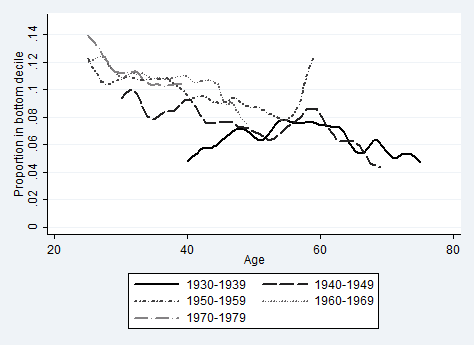
\includegraphics[width=.5\linewidth]{pictures/cohortagerisksmooth_bhc_inc.png} &
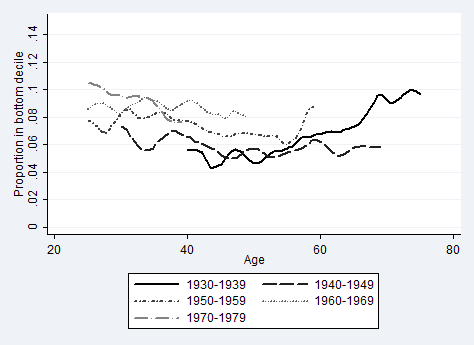
\includegraphics[width=.5\linewidth]{pictures/cohortagerisksmooth_bhc_con.png} \\
(a) Income inc. Housing & (b) Consumption inc. Housing \\
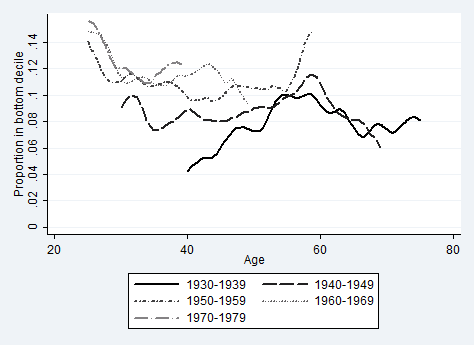
\includegraphics[width=.5\linewidth]{pictures/cohortagerisksmooth_ahc_inc.png} &
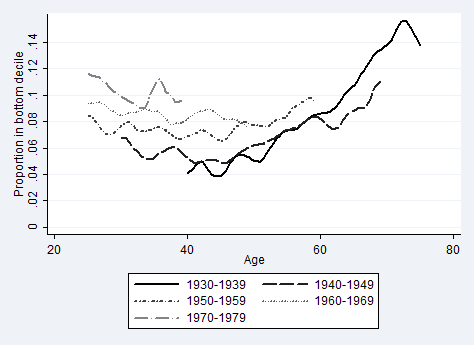
\includegraphics[width=.5\linewidth]{pictures/cohortagerisksmooth_ahc_con.png} \\
(c) Income ex. Housing & (d) Consumption ex. Housing \\
\end{tabular}
\label{fig:povage_cohort}
\end{figure}

\begin{figure}
\caption{Risk of Poverty, by Age and Cohort }
\centering
\begin{tabular}{c c}
Income & Consumption\\
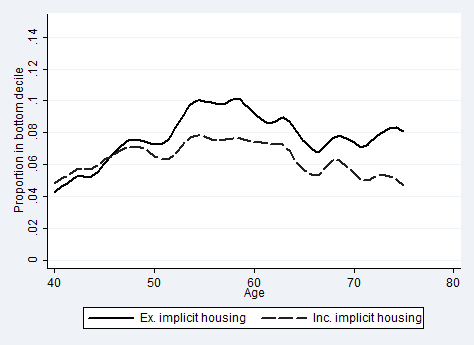
\includegraphics[width=.5\linewidth]{pictures/cohort2_agerisksmooth_inc.png} &
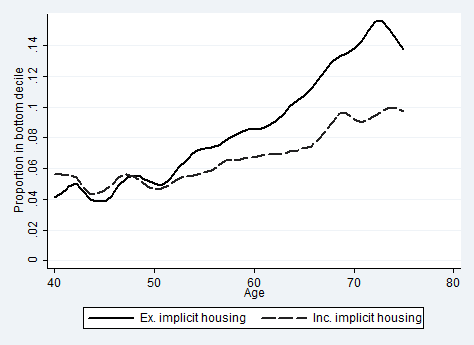
\includegraphics[width=.5\linewidth]{pictures/cohort2_agerisksmooth_con.png} \\
(a) 1930s Cohort & (b) 1930s Cohort \\
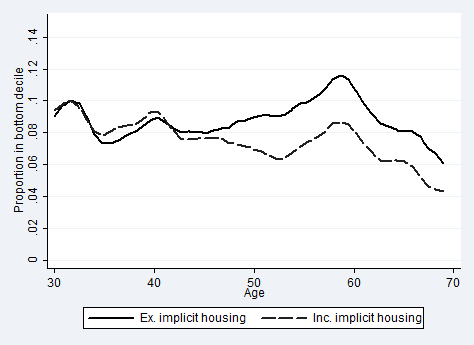
\includegraphics[width=.5\linewidth]{pictures/cohort3_agerisksmooth_inc.png} &
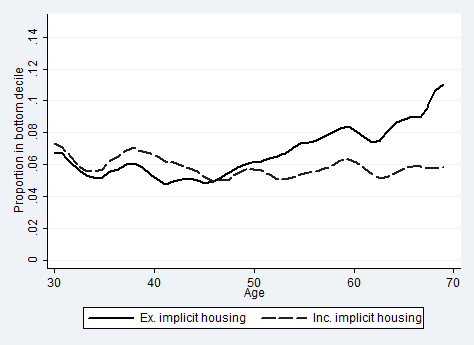
\includegraphics[width=.5\linewidth]{pictures/cohort3_agerisksmooth_con.png} \\
(c) 1940s Cohort & (d) 1940s Cohort \\
\end{tabular}
\label{fig:povage_cohort_restrict}
\end{figure}


\begin{figure}
\caption{Average Rooms Occupied per Person}
\centering
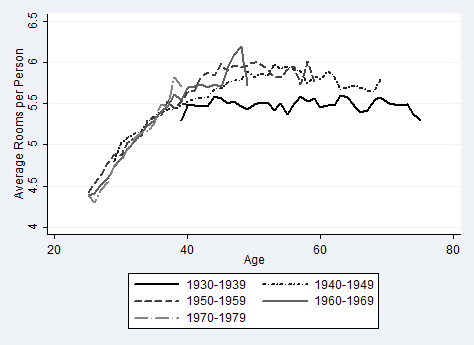
\includegraphics[width=.7\linewidth]{pictures/cohort_rooms.png}
\label{fig:cohort_rooms}
\end{figure}

\begin{figure}
\caption{Average People in Household}
\centering
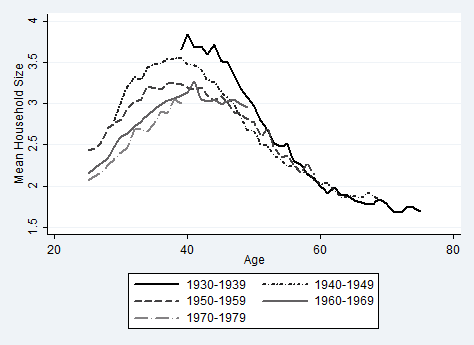
\includegraphics[width=.7\linewidth]{pictures/av_peep.png}
\label{fig:cohort_peeps}
\end{figure}


\begin{figure}
\caption{Average Rooms per Person, 1979-2000}
\centering
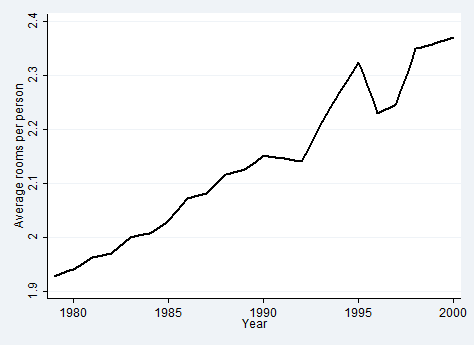
\includegraphics[width=0.7\linewidth]{pictures/rooms_pp.png}
\label{fig:room_time}
\end{figure}



